\thispagestyle{doisongtoanhocnone}
\pagestyle{doisongtoanhoc}
\everymath{\color{doisongtoanhoc}}
\graphicspath{{../doisongtoanhoc/pic/}}
\blfootnote{$^1$\color{doisongtoanhoc}Theo thông báo Viện Hàn lâm Khoa học và Văn học Na Uy. https://abelprize.no/article/2023/luis-caffarelli-awarded-2023-abel-prize}
\begingroup
\AddToShipoutPicture*{\put(0,616){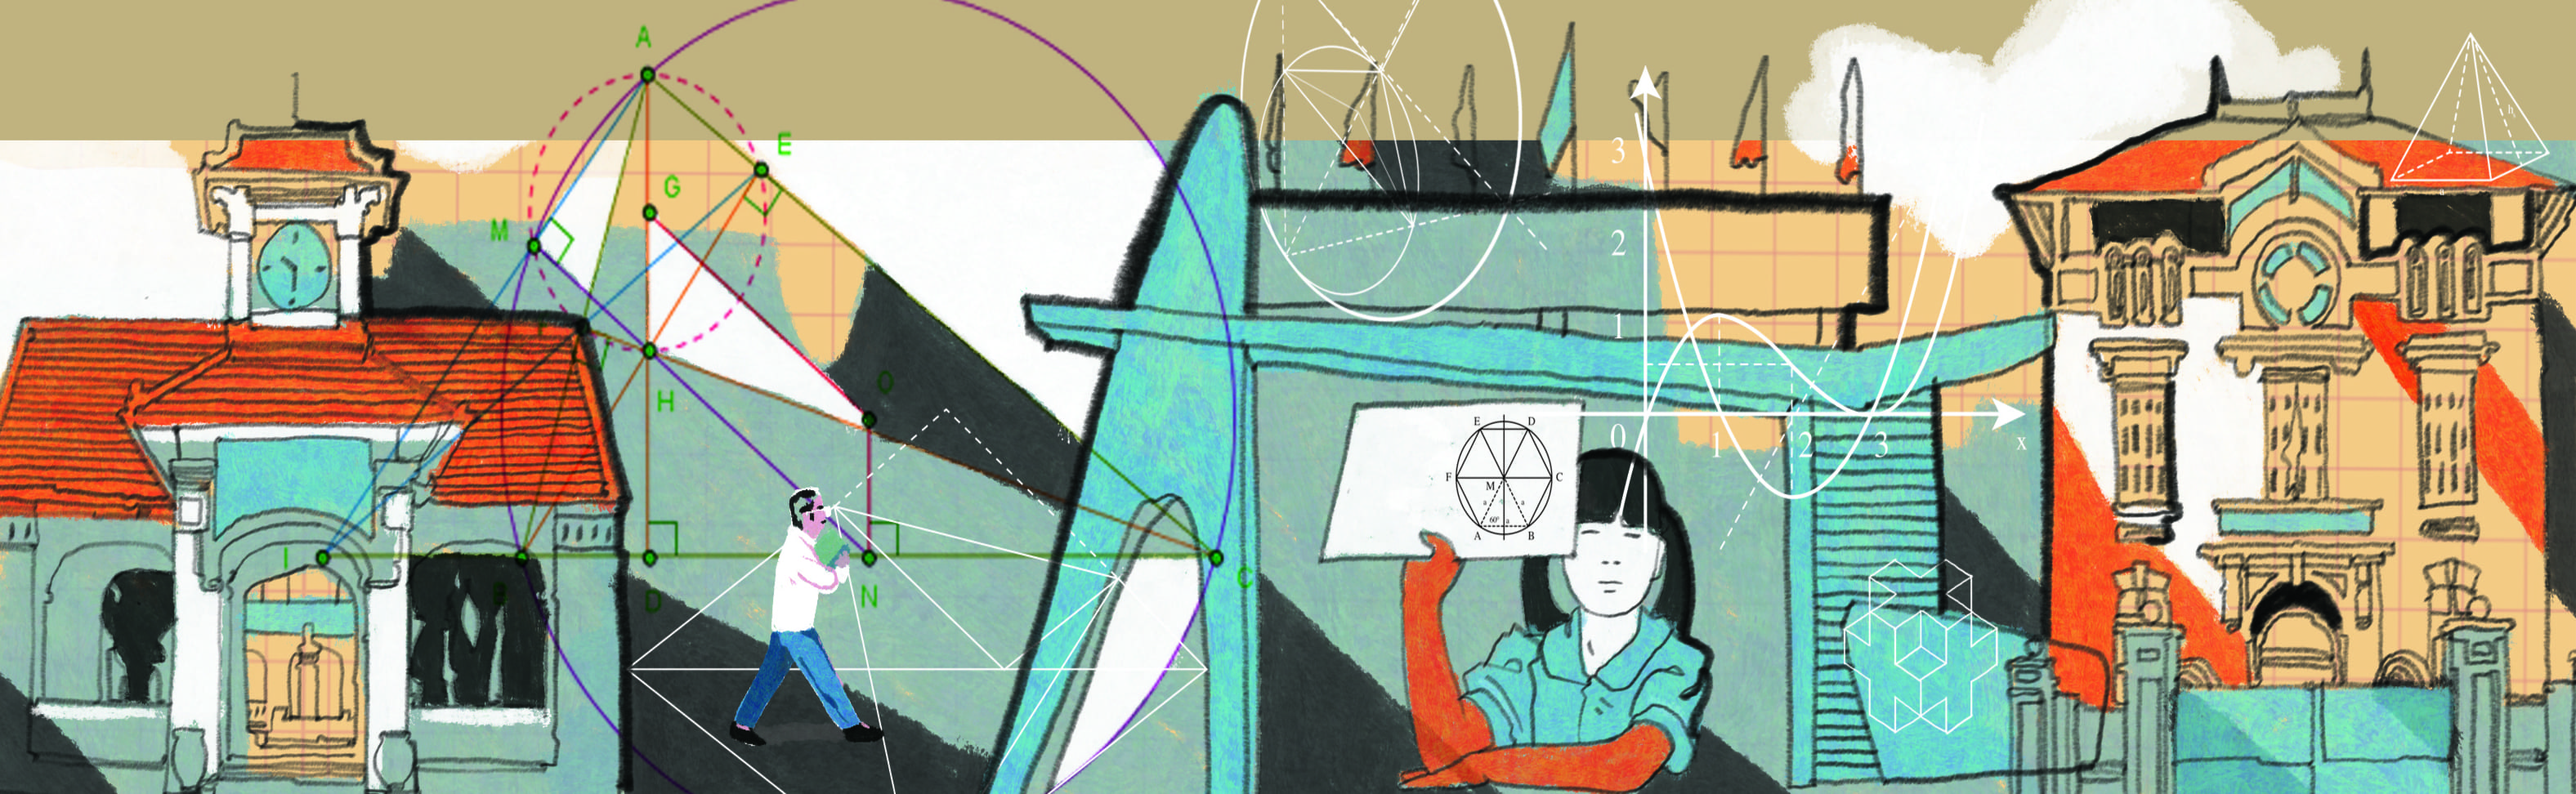
\includegraphics[width=19.3cm]{../bannerdoisong}}}
\AddToShipoutPicture*{\put(100,555){
\includegraphics[scale=0.95]{../tieude.pdf}}}\centering
\endgroup

\vspace*{150pt}


\begin{multicols}{2}	
	Luis A. Caffarelli được trao tặng Giải thưởng Abel $2023$ vì ``những đóng góp đầy sức ảnh hưởng vào lý thuyết chính quy cho  các phương trình đạo hàm riêng phi tuyến bao gồm các bài toán không có biên và phương trình Monge–Ampère.".
	\begin{figure}[H]
		\vspace*{-5pt}
		\centering
		\captionsetup{labelformat= empty, justification=centering}
		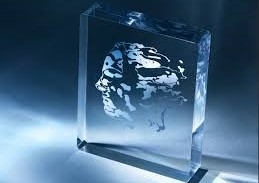
\includegraphics[width= 1\linewidth]{1}
		\vspace*{-15pt}
	\end{figure}
	Phương trình vi phân là công cụ mà các nhà khoa học sử dụng để dự đoán hành vi của thế giới vật chất. Các phương trình này liên hệ một hoặc nhiều hàm số chưa biết và các đạo hàm của chúng. Các hàm số này thường đại diện cho các đại lượng vật lý, các đạo hàm đại diện cho tỷ lệ thay đổi của chúng và phương trình vi phân định nghĩa một mối quan hệ giữa hai đại lượng này. Những mối quan hệ như vậy là phổ biến; do đó, các phương trình vi phân đóng một vai trò nổi bật trong nhiều ngành bao gồm kỹ thuật, vật lý, kinh tế, và sinh học.
	\vskip 0.1cm
	Các phương trình đạo hàm riêng phát sinh một cách tự nhiên như các quy luật của Tự nhiên, để mô tả các hiện tượng khác nhau như dòng chảy của nước hoặc sự phát triển của dân số. Những phương trình này luôn là khởi nguồn của những nghiên cứu mạnh mẽ kể từ thời của Isaac Newton và Gottfried Leibniz. Tuy nhiên, bất chấp những nỗ lực đáng kể của nhiều nhà toán học trong nhiều thế kỷ, các câu hỏi cơ bản liên quan đến sự tồn tại, tính duy nhất, tính chính quy, và tính ổn định của các nghiệm của một số phương trình chủ chốt vẫn chưa được giải quyết.
	\begin{figure}[H]
		\vspace*{-5pt}
		\centering
		\captionsetup{labelformat= empty, justification=centering}
		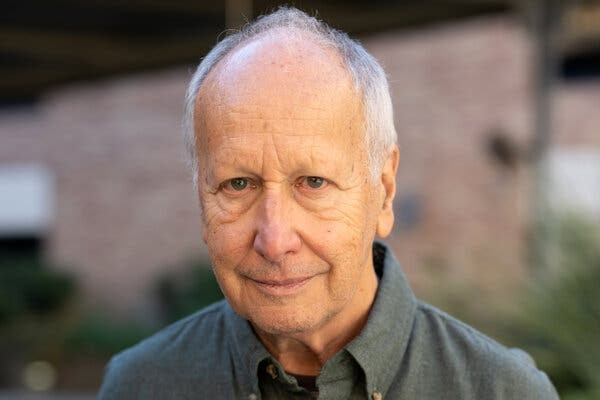
\includegraphics[width= 1\linewidth]{2}
		\caption{\small\textit{\color{doisongtoanhoc}Bản quyền ảnh: Nolan Zunk, Đại học Texas ở Austin.}}
		\vspace*{-10pt}
	\end{figure}
	\textbf{\color{doisongtoanhoc}Kết quả chuẩn mực về kỹ thuật}
	\vskip 0.1cm
	Rất ít nhà toán học đương đại khác có đóng góp nhiều hơn so với Luis Caffarelli, một người Mỹ gốc Argentina, cho sự hiểu biết của chúng ta về phương trình đạo hàm riêng. Ông đã đưa ra những kỹ thuật mới tài tình, thể hiện cái nhìn sáng suốt về hình học và tạo ra nhiều kết quả có sức ảnh hưởng. Trong khoảng thời gian hơn $40$ năm, ông đã có những đóng góp đột phá cho lý thuyết về tính chính quy. Tính chính quy -- hay độ trơn -- của các nghiệm là thiết yếu trong những tính toán số, và sự vắng mặt của tính chính quy là thước đo mức độ hoang dã mà Tự nhiên có thể hành xử.
	\vskip 0.1cm
	Helge Holden, chủ tịch Ủy ban Abel, cho biết: ``Các định lý của Caffarelli đã thay đổi hoàn toàn hiểu biết của chúng ta về các lớp phương trình đạo hàm riêng phi tuyến với nhiều ứng dụng. Các kết quả là chuẩn mực về mặt kỹ thuật, ảnh hưởng tới nhiều lĩnh vực khác nhau của toán học và các ứng dụng của nó." 
	\vskip 0.1cm
	Phần lớn công việc của Luis A. Caffarelli liên quan đến các bài toán không có biên.  Ví dụ, hãy xem xét vấn đề băng tan thành nước. Ở đây biên tự do là giao diện giữa nước và băng; nó là một phần của ấn số cần được xác định. Một ví dụ khác là nước thấm qua một môi trường xốp -- một lần nữa, giao diện của nước và môi trường cần được hiểu rõ. Caffarelli đã đưa ra các giải xuyên thấu cho những vấn đề này với các ứng dụng cho các giao diện rắn--lỏng, dòng phun và tạo bọt, dòng khí và dòng chảy chất lỏng trong môi trường xốp, cũng như toán tài chính.
	\vskip 0.1cm
	\textbf{\color{doisongtoanhoc}Ảnh hưởng to lớn đến lĩnh vực}
	\vskip 0.1cm
	Caffarelli là một nhà toán học có hiệu suất đặc biệt, với hơn $130$ cộng sự và hơn $30$ nghiên cứu sinh trong khoảng thời gian $50$ năm.
	\vskip 0.1cm
	Helge Holden nói: ``Nhờ kết hợp sự hiểu biết sáng suốt về hình học với các công cụ và phương pháp giải tích khéo léo, ông [Caffarelli] đã và tiếp tục có ảnh hưởng to lớn đến lĩnh vực này."
	\vskip 0.1cm
	Luis A. Caffarelli đã giành được nhiều giải thưởng, trong đó có Giải thưởng Leroy P. Steele cho Thành tựu Trọn đời về Toán học, Giải thưởng Wolf và Giải thưởng Shaw.
\end{multicols}
\vspace*{-10pt}
{\color{doisongtoanhoc}\rule{1\linewidth}{0.1pt}}

\vspace*{5pt}
\centerline{\Large\textbf{\color{doisongtoanhoc}LỜI GIẢI, ĐÁP ÁN}}

\vspace*{-5pt}
\begin{multicols}{2}
	\textbf{\color{doisongtoanhoc}Đố vui}
	\vskip 0.1cm
	$a)$ Sau khi Bình buộc $2$ đầu dây tại một bên của nắm tay, ta có tình huống như sau:
	\begin{figure}[H]
		\vspace*{-10pt}
		\centering
		\captionsetup{labelformat= empty, justification=centering}
		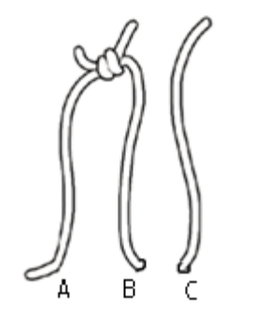
\includegraphics[scale=0.3]{do_vui_1}
		\vspace*{-10pt}
	\end{figure}
	Khi Bình buộc hai đầu ở phía bên còn lại của nắm tay, bạn sẽ nối $A$ với $B$ hoặc $B $ với $C$, hoặc $A$ và $C$. Như vậy, có hai trong ba trường hợp các đoạn dây được buộc lại thành một đoạn dây, nghĩa là xác suất cần tìm là $\dfrac{2}{3}$.
	\vskip 0.1cm
	$b)$ Sau khi Bình buộc $2$ cặp đầu dây tại một bên của nắm tay, ta có tình huống như sau:
	\begin{figure}[H]
		\vspace*{-2pt}
		\centering
		\captionsetup{labelformat= empty, justification=centering}
		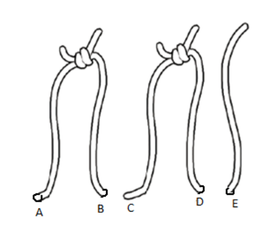
\includegraphics[scale=0.42]{do_vui_2}
		\vspace*{-10pt}
	\end{figure}
	Tiếp theo, ta có thể lập luận tương tự như $a)$ bằng cách đếm tất cả các tổ hợp buộc $2$ cặp đầu dây giữa $A, B, C, D$ và $E$. Tuy nhiên, để tránh nhàm chán, ta sẽ lập luận khác đi, như sau. Để ý rằng, với mọi cách buộc $2$ cặp đầu dây ở phía còn lại của nắm tay, sẽ có đúng một đầu tự do (không bị buộc); trong đó cách buộc duy nhất khiến cho có một đoạn dây không được buộc với bất kỳ đoạn nào khác là đầu tự do là $E$. Vì xác suất để đầu $E$ là tự do bằng $\dfrac{1}{5}$ nên đáp số là $\dfrac{1}{5}$.
	\vskip 0.1cm
	
\end{multicols}